\chapter{Речка Дарница}

Я много упоминал речку Дарницу, так что придется рассказать о ней подробнее. Дарнице посвящена отдельная серия «Киевской амплитуды», но когда мы снимали ее, то не видели еще старинной польской карты\footnote{Эту карту 1640 года я по сей день хорошо не рассмотрел. У меня есть кусок в хорошем качестве, и полный скан в качестве отвратительном.}, где четко обозначена эта река, и предполагали исток около Княжичей, в Ялынке, а на деле его следует искать в Броварах или к северо-востоку от них. А может, того истока уже нет и он сместился к Ялынке.

Вообще имя Дарницы носила и местность (причем одноименная станция метро не имеет к ней  отношения), и огромное озеро, и речка – эта глава посвящена больше именно последней.

Помню, снимали мы про Дарницу долго, много разрозненных съемочных дней, почти всё лето 2013 года, самого плодовитого на серии. Пешие походы по жаре, и в тени через комариный рай, и лесом на велосипеде.

Река Дарница раскинулась по всему Левому берегу и нельзя за один присест ее обойти. Ни над одной рекой так не издевались – и отходами загаживали, и на части разделяли, а сейчас кое-кто вовсе отказывает ей в историческом существовании – мол, нет такой речки, есть Северодарницкий мелиоративный канал.

А ведь прежде всё было иначе. Жила-была речка Дарница. Вот она на той самой польской карте:

\begin{center}
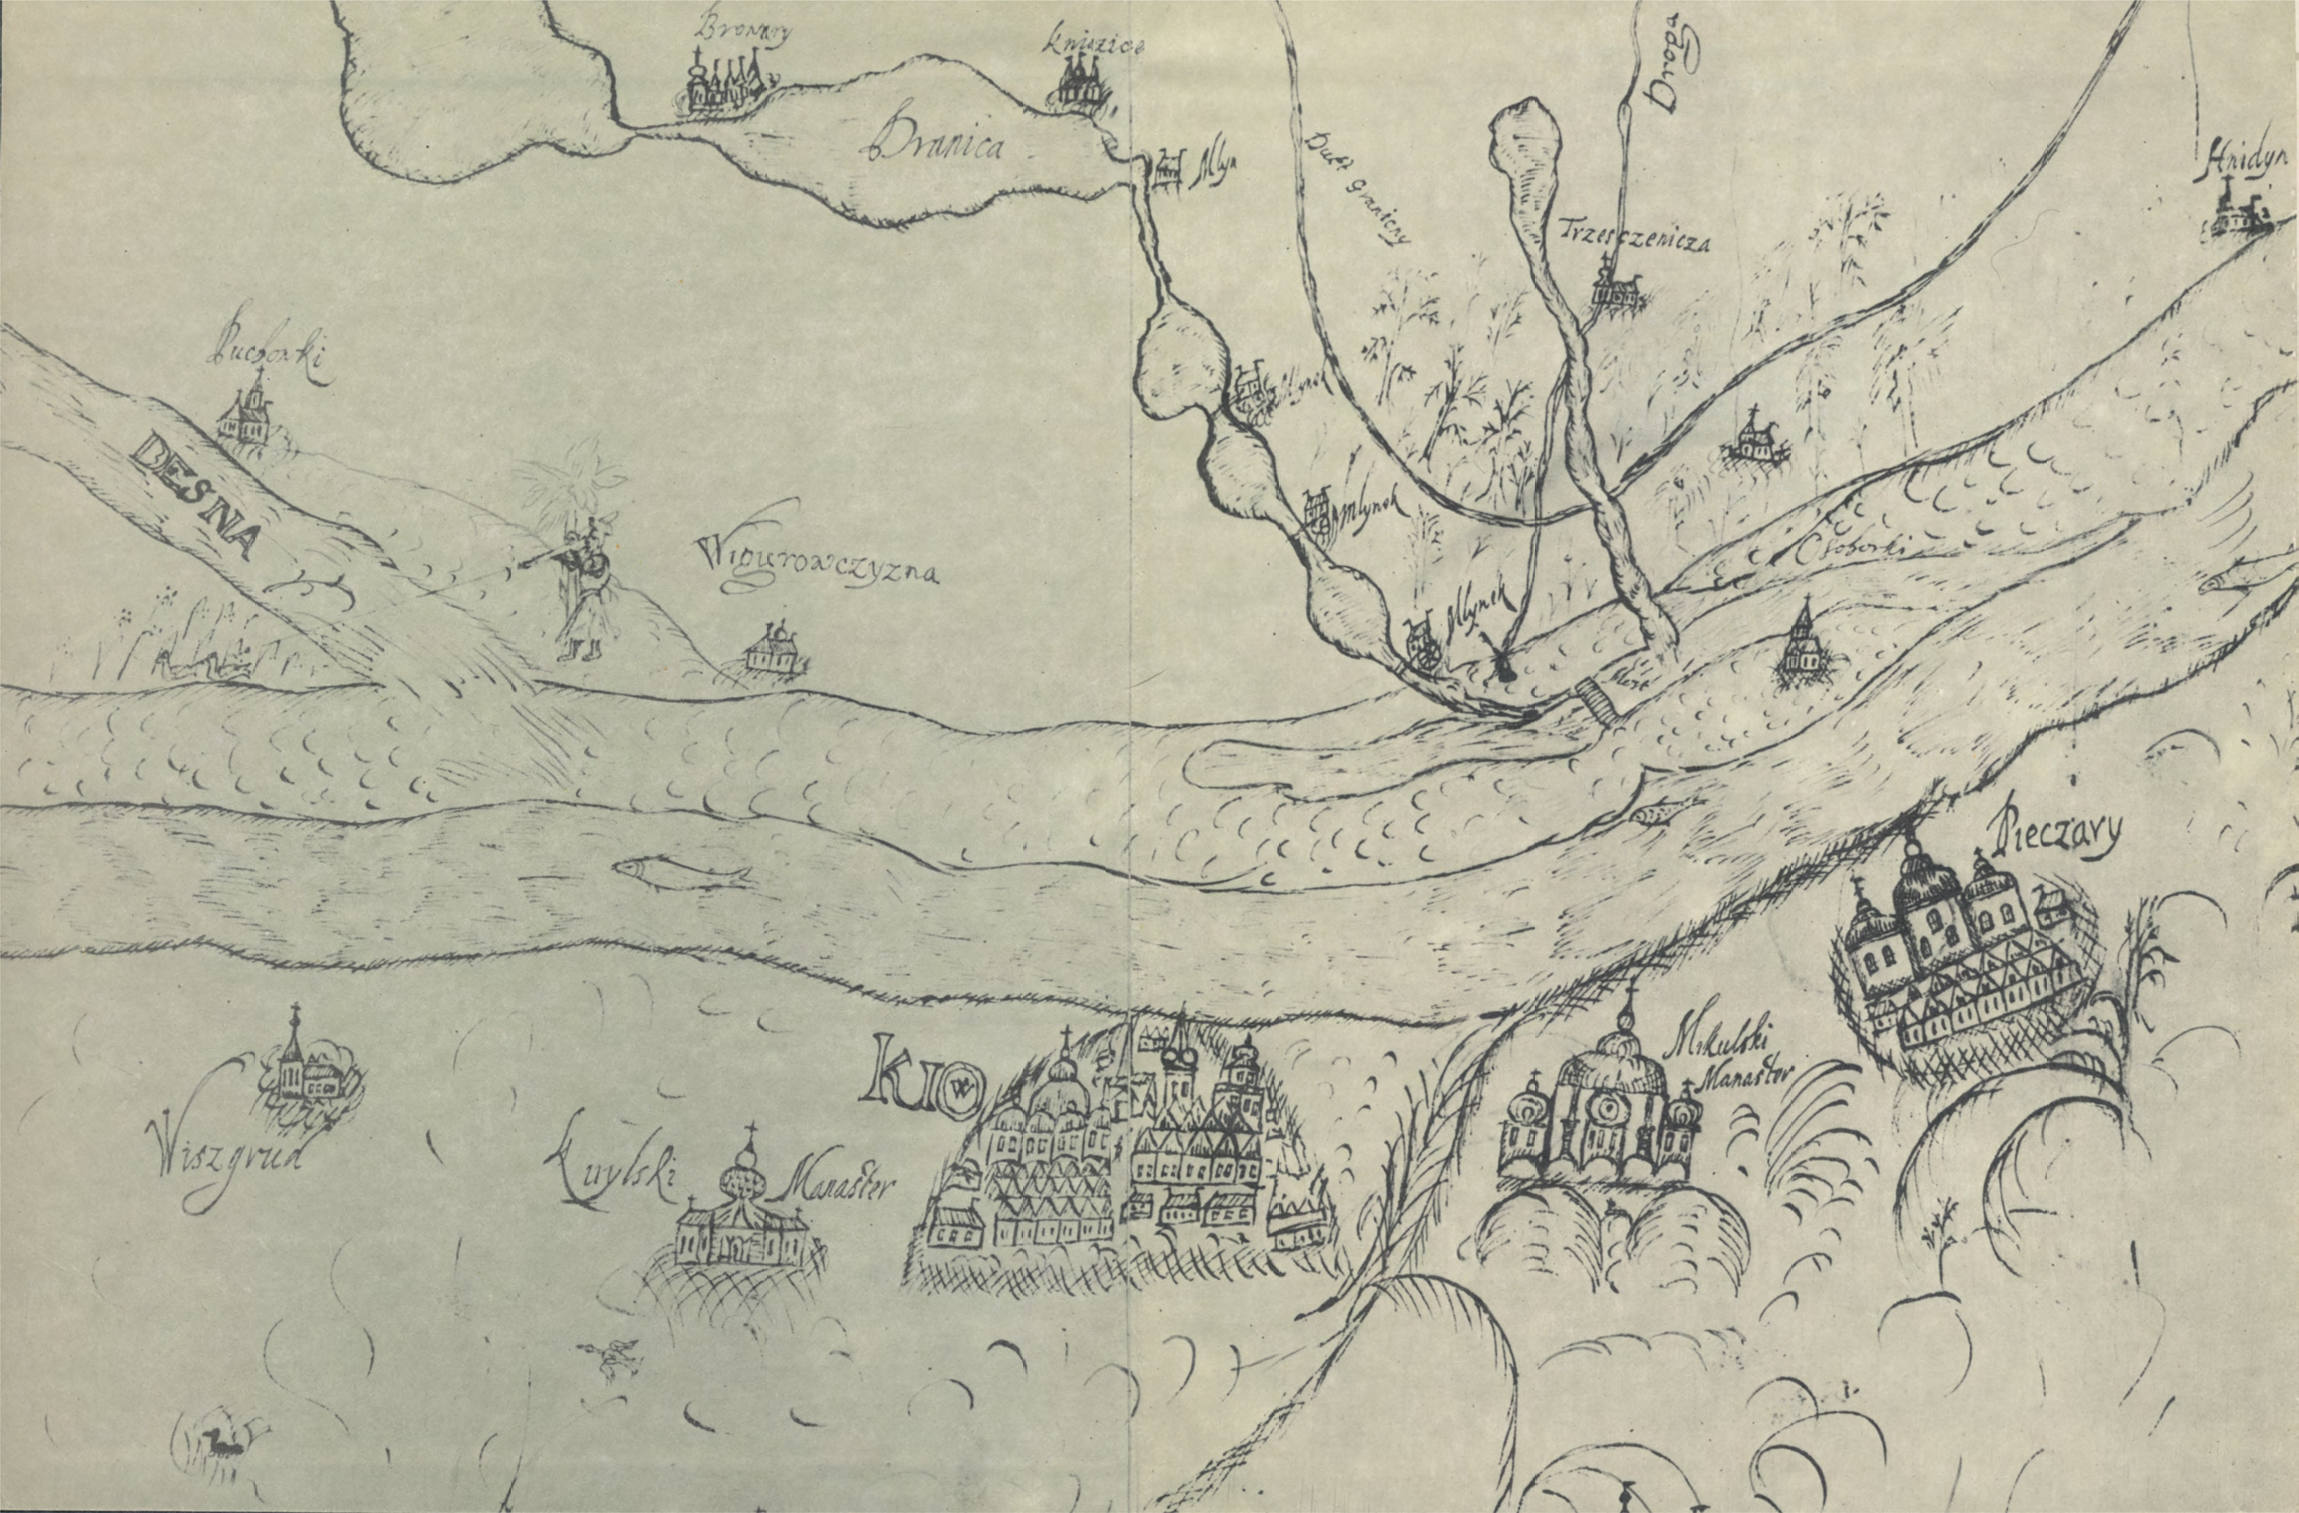
\includegraphics[width=\linewidth]{chast-gorodki/darn/s_1992-kroynika.jpg}
\end{center}

Дарница подписана здесь как «Dranica». В верхней левой части два населенных пункта – Бровары и Княжичи. Дарница протекает мимо них, в виде двух наверное прудов, очень раздутая, почти как Днепр. Ничего удивительного в этом нет, подобные пруды по сей день находятся на речке Борщовке.

В Броварах есть несколько разрозненных озер, и одно из наибольших – в парке Победы. Юго-восточная часть парка стоит на костях, там было еврейское кладбище, и поваленные надгробия встречались еще в начале двухтысячных. Если залезть в парке на курган и смотреть в сторону, противоположную от озера, на рощу – там и было кладбище. Я плохо знаком с прошлым Броваров, поэтому не знаю, что это за озеро. В конце 1980-х в парке был наполненный водой бетонный канал, вдоль улицы Воссоединения, со стороны улицы Гагарина. Словом, броварской след в происхождении Дарницы для меня неясен.

Изображенная на польской карте толстая часть Дарницы от Броваров до Княжичей, на трехверстовках Шуберта середины 19 века превратилась уже в подобное луговой реке «озеро Свидловщину», к востоку от коего распространилось болото. Свидловщина близ северо-западной границы Княжичей поворачивало на запад к железной дороге да озеру Рыбному. Сейчас на отрезке от Броваров до Княжичей – район Княжичей Ялынка, прежде бывшая дачным поселком. Там есть одноименная железнодорожная станция. Дома между нею и Княжичами называют Ялынкой, но по адресам улицы последней относятся ко Княжичам.

\begin{center}
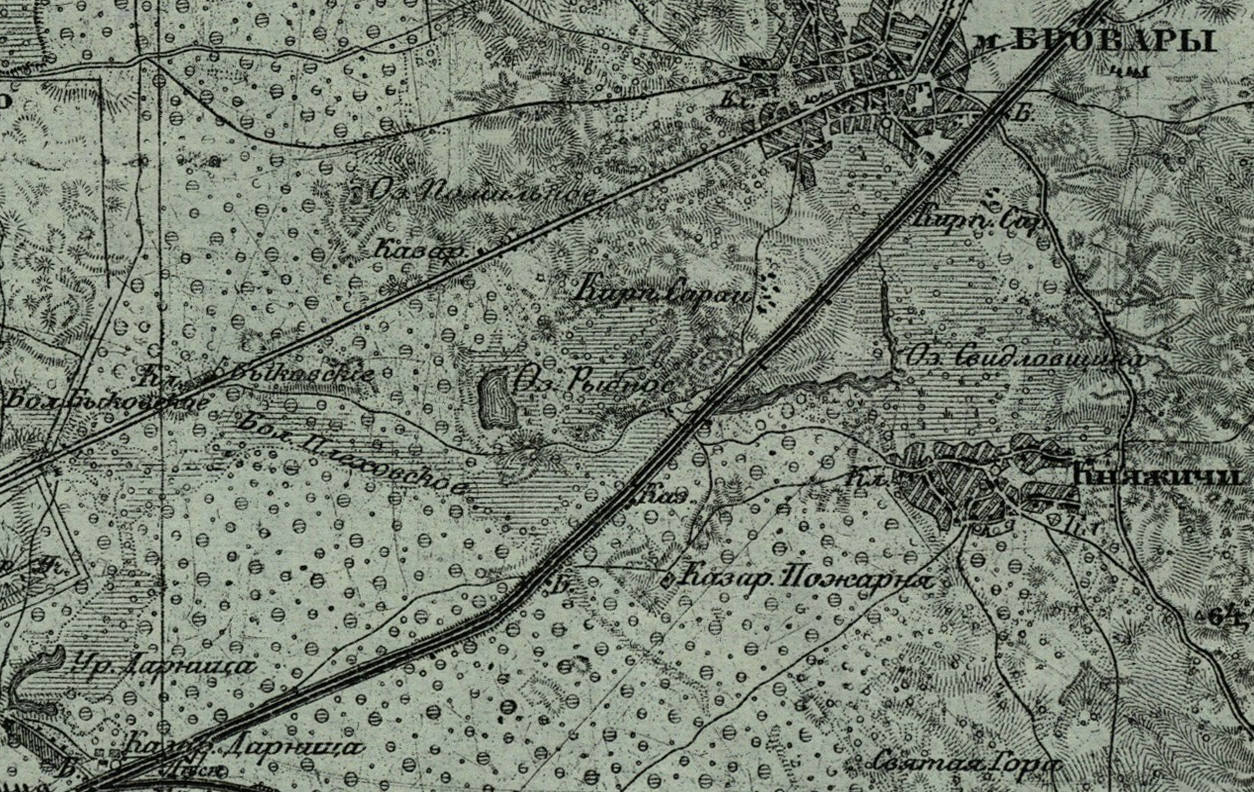
\includegraphics[width=\linewidth]{chast-gorodki/darn/s_1850-darn.jpg}
\end{center}

Дарница в образе Свидловщины огибает Ялынку по восточной, затем по северной границе эдак до 7-й Садовой улицы. Вода почти всюду покрыта зеленой ряской.

Ялынка весьма точно вписывается между Свидловщиной и железной дорогой. Далее вода Дарницы течет ручьем южнее озера Рыбного, образуя по пути каскад озер и болотец. Какую роль озеро Рыбное играет в этой водной системе, не знаю. Затихшее, огромное – полкилометра на четыреста метров, пусто раскинулось в лесной плеши лесом рядом с «быковнянскими могилами» (они кстати гораздо ближе к хутору Рыбному, чем к Быковне) и заброшенными строениями свинофермы. Издалека видно тамошнюю водонапорную башню.

В 2013 году я, вооружившись видеокамерой и фотыком, на велосипеде отправился исследовать участок Дарницы в том краю. Повернув на север от Броварского шоссе, безлюдной дорогой через лес поехал к хутору Рыбному. Улица, несколько домиков, рядом припаркованы машины. Несколько местных во дворах. Играющие дети. Колесить по хутору мне не хотелось, в памяти возникли шаблонные американские фильмы ужасов, где одинокий путник, сбившись с пути, попадает в захолустный городок, жители коего настороженно смотрят из окон. Неподалеку, я знал по карте, расположена скотобойня. Поддал крутить педали.

Дорогу к Рыбному озеру я тогда не нашел. В лесу разбегалось много бугристых дорог, все грунтовые, точнее из плотно сбитого песку, и даже мой огромный дорожник «Аист» отчаянно буксовал. GPS, как обычно, не хотел запускаться, поэтому на перекрестках я руководствовался наитием. Наитие привело меня к болоту, откуда я услыхал шум проходящих поездов и понял, что если буду следовать на него, не пропаду. Я залез на сухое дерево над болотом, поснимал водную гладь, затем вжарил скорость, обогнав двух туристов. Сбоку возник песчаный косогор. На верху росли сосны.

Где-то здесь, в окрестностях Ялынки, в восьмидесятых годах мы с отцом катались на великах. Я был мал, и велосипед мой был мал – складной «Минск» (потом его называли «Аистом»). Тогда мы попали под ливень и размокшими дорогами пробивались назад к электричке.

А сейчас я понял, что заблудился. Поезда перестали свистеть. Впереди шла женщина лет сорока-пяти, с корзиной, в спортивных штанах и вязаной кофте на голое тело. Небось собирала в лесу разное зелье. Я спросил, как проехать к железной дороге, женщина стала обстоятельно рассказывать, как удобнее, особенно на велосипеде, но я ничего не понял, поблагодарил и стал вкручивать педали дальше.

Хвойный лес сменился лиственным. Я достигнул гати через Дарницу, что текла под насыпью через несколько ржавых труб. По обе стороны дороги было довольно приличное русло, а вот водичка едва покрывала дно, растекаясь по ширине. Около труб прыгали маленькие коричневые лягушки.

Я последовал вдоль русла, сколько мог с велосипедом, а затем выбрался таки к железной дороге (как понимаю теперь, в урочище Мостище, чье имя указывает на давний мост), но до самой Ялынки не поехал, отложив на потом. Вместо этого покатил рядом с рельсами весьма неудобной тропкой.

Вся эта местность называлась Плеховским болотом. Вот во что превратились пруды, на которых стояли водяные мельницы. В наше время болото несколько усохло и от железной дороги отдалилось. Сквозь жутковатую чащу я его не видел. Долго ли, коротко, свернул наобум вправо. Там и нашел остатки прудов. Места эти своей безлюдностью и вместе с тем ощущением чьего-то присутствия, некоего ожидания, напоминают мне фильм «Пикник у Висячей скалы».

От Ялынки руслу Дарницы придан вид ломаной линии – она давно уже не петляет обычной полевой рекой, но сочится по спрямленным участкам русла, наполняя пруды.

Из пруда в пруд вода с шумом перетекает через трубы:

\begin{center}
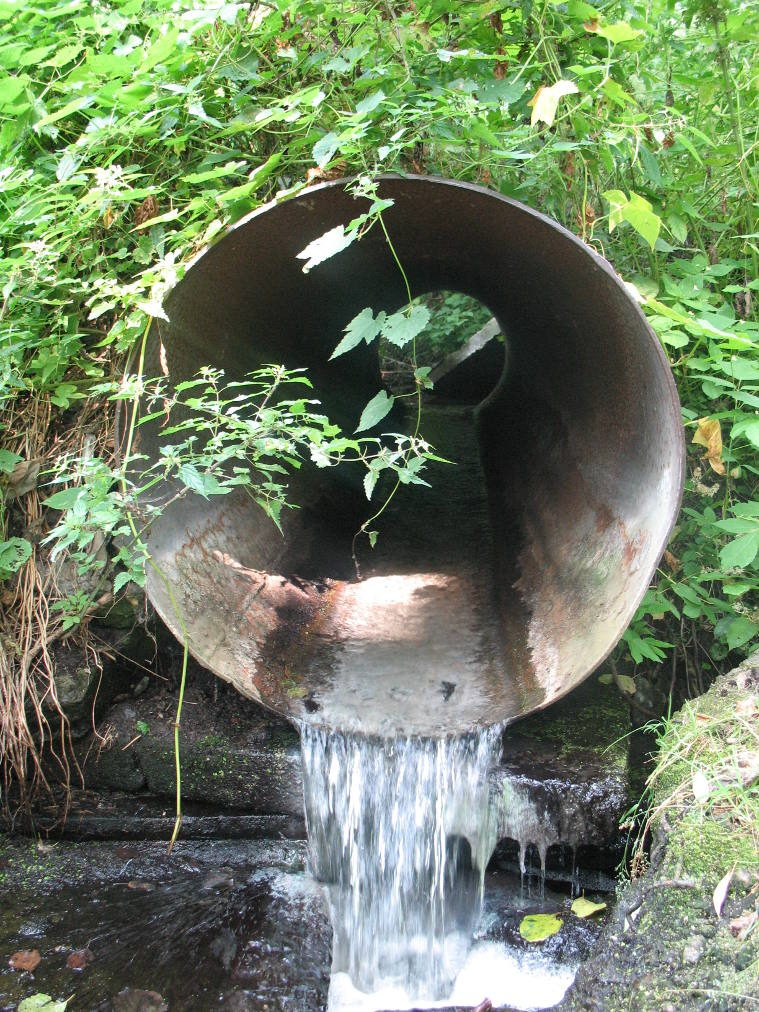
\includegraphics[width=0.51\linewidth]{chast-gorodki/darn/s_darn-IMG_2747.JPG}
\end{center}

\newpage
\vspace*{\fill}
\begin{center}
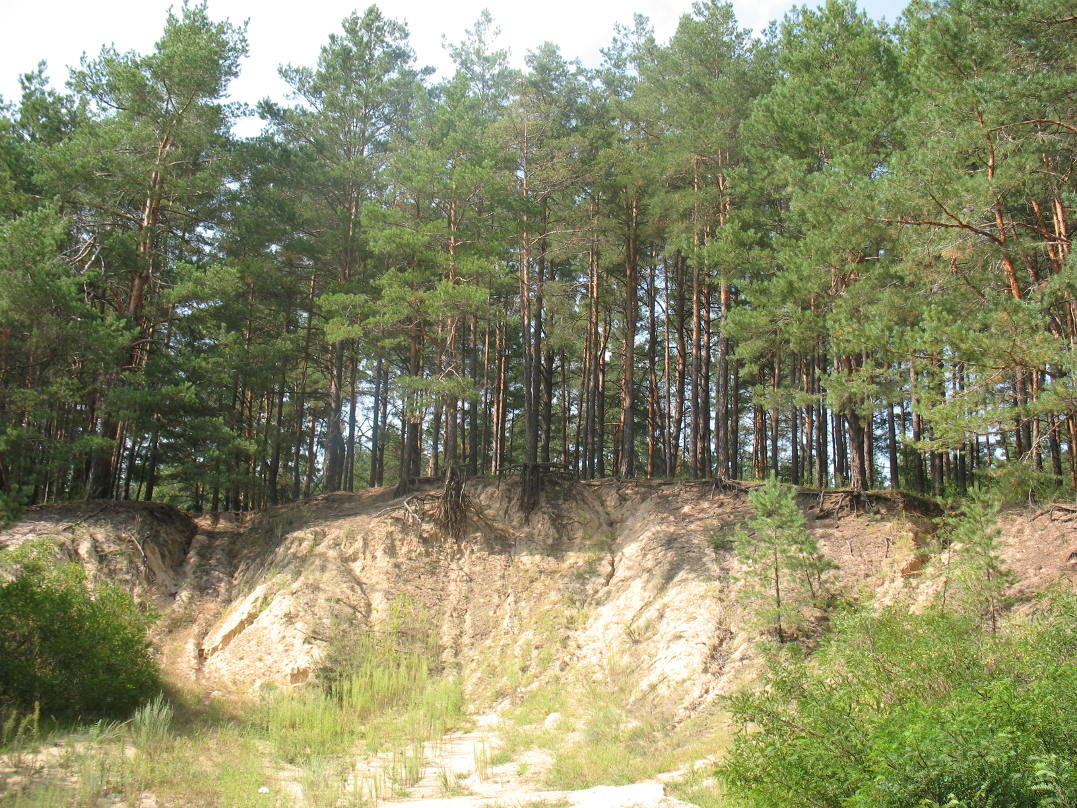
\includegraphics[width=\linewidth]{chast-gorodki/darn/s_darn-IMG_2743.JPG}
\end{center}

\begin{center}
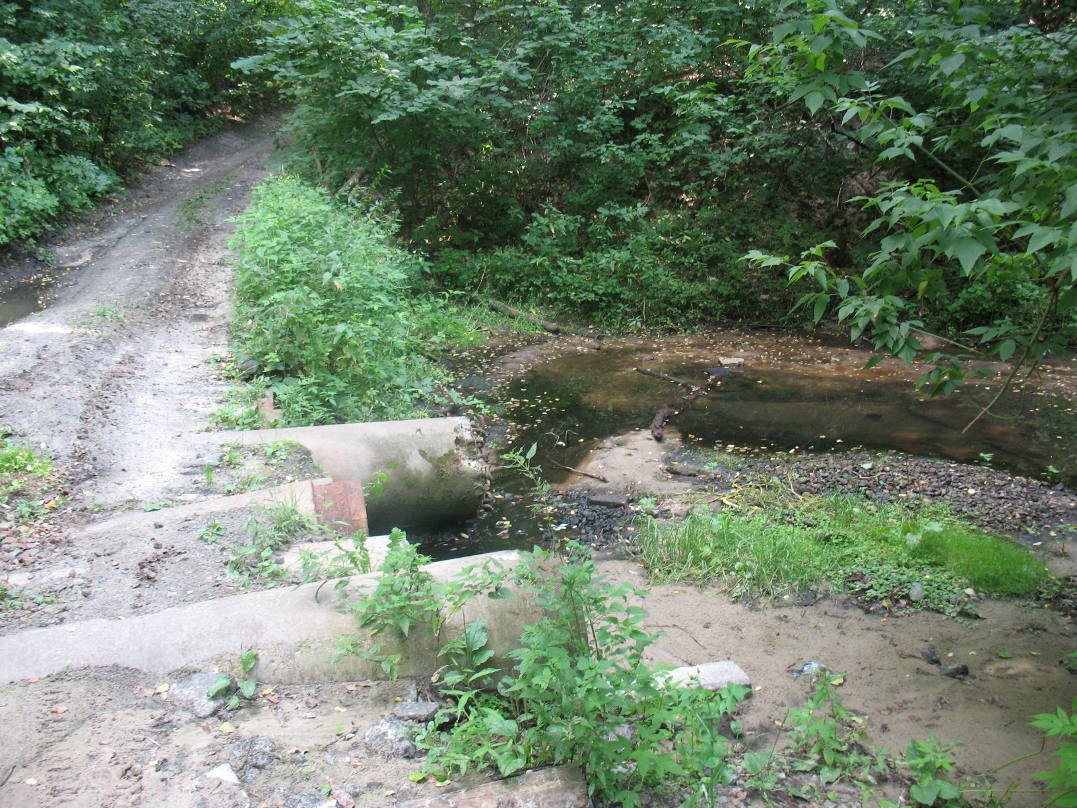
\includegraphics[width=\linewidth]{chast-gorodki/darn/s_darn-IMG-2745.JPG}
\end{center}
\vspace*{\fill}
\newpage
\vspace*{\fill}
\begin{center}
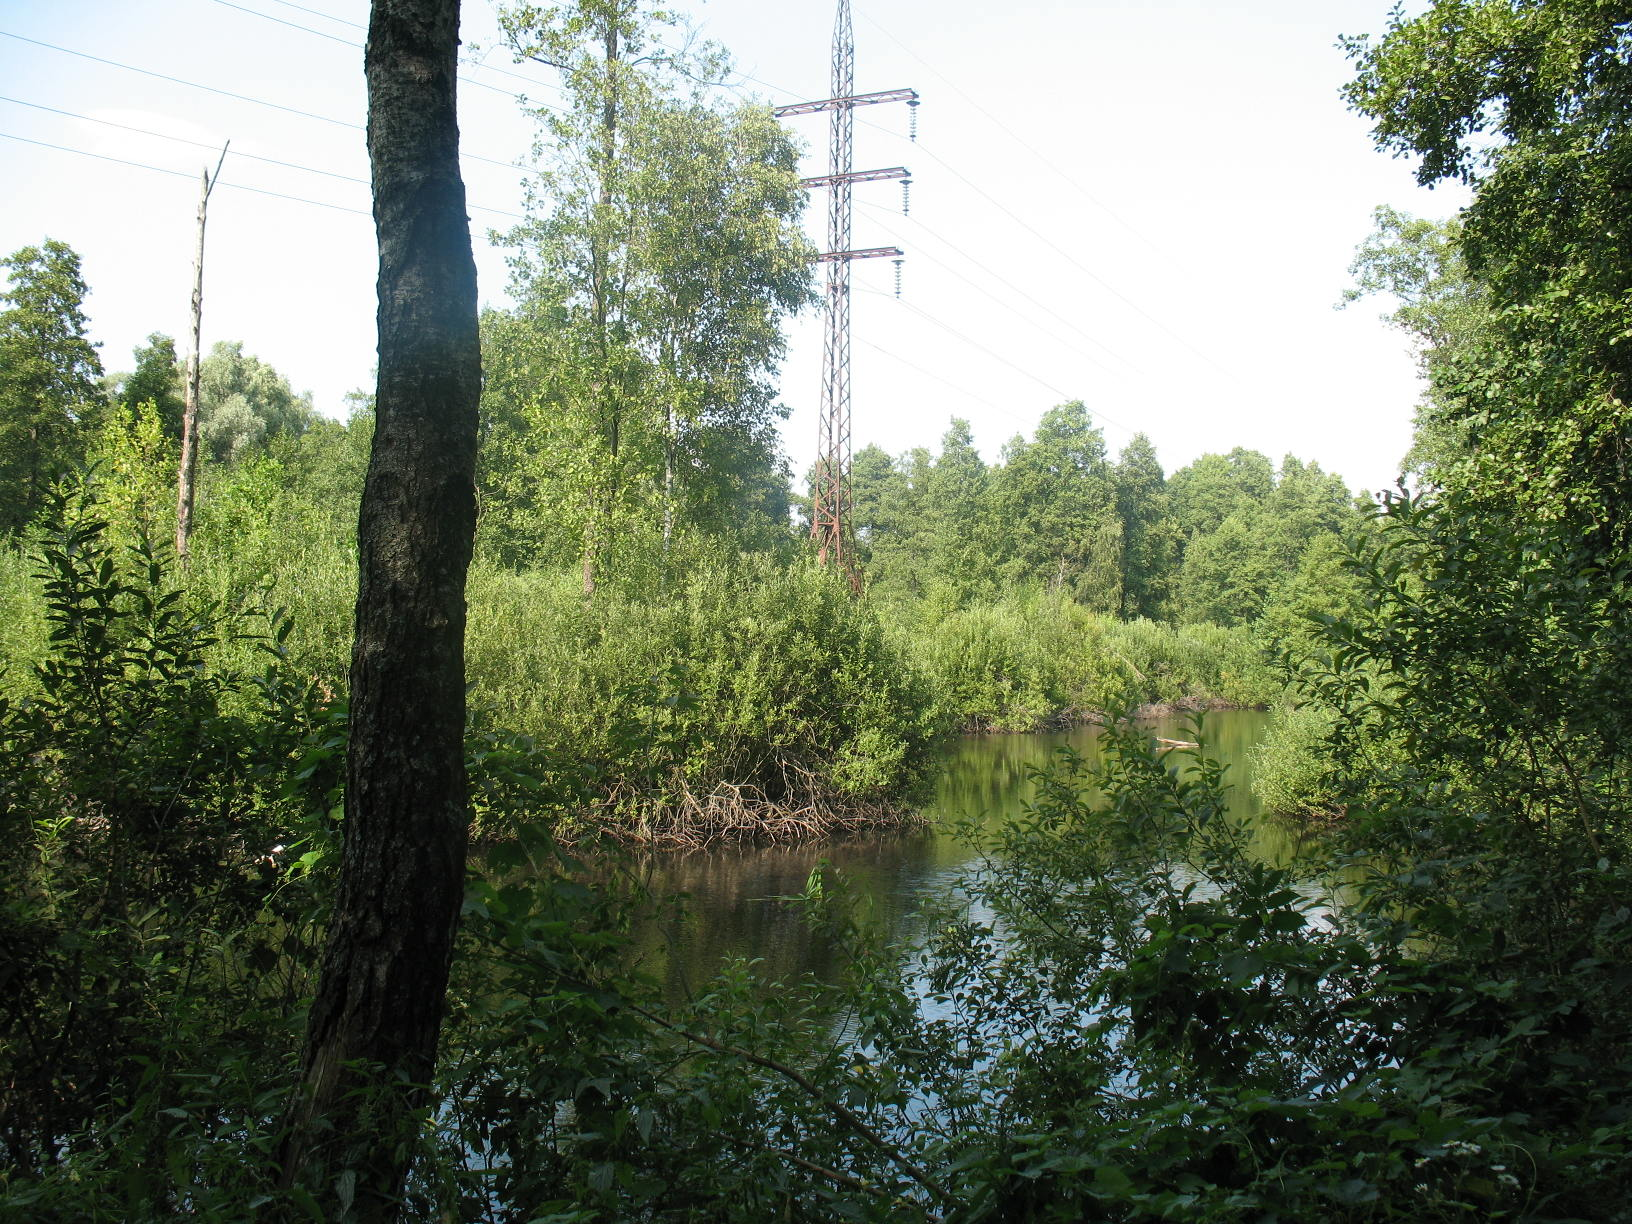
\includegraphics[width=\linewidth]{chast-gorodki/darn/s_darn-IMG_2756.JPG}
\end{center}

\begin{center}
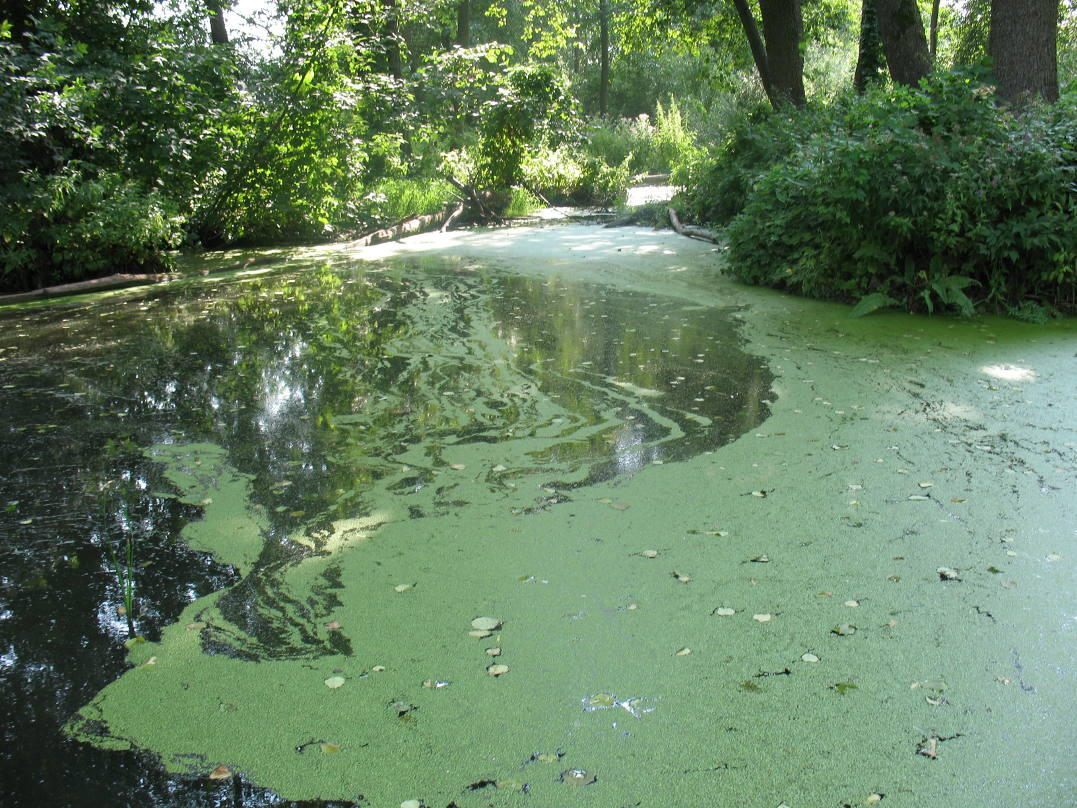
\includegraphics[width=\linewidth]{chast-gorodki/darn/s_darn-IMG_2751.JPG}
\end{center}
\vspace*{\fill}
\newpage

Вот так и прежде – были пруды, а при них заводились мельницы, что способствовало обмелению Дарницы и заболачиванию прилегающих земель. Документально мельницы известны на Дарнице еще с начала 16 века. 

В решении межевого суда о границах владений Печерского и Николо-Пустынного монастырей на земле Зверинской, 1508 года сказано\cite[том 4, часть 8, стр. 160]{akty02}:

\begin{quotation} 
реку Дарницу, на которой же реце и млынища, што перед тым стого\footnote{Стого – святого.} Николы Пустынского млын был, и на тои гребле есмо стояли [...] тое дей млынищо и с тым озером гдрское\footnote{Господарское.} нам жалование
\end{quotation} 

Млынище (место прежней мельницы) на речке Дарнице упомянуто и в грамоте 1516 года. Проходит 200 лет, а реку всё используют, чтобы крутить колеса мельниц. В жалованной грамоте в Киевопечерскую Лавру на владения Троицкому Больницкому монастырю, 1720 года, записана «мельница Дарницкая нижняя»\footnote{Возможно, она стояла к юго-востоку от нынешней Дарницкой ТЭЦ – возле нее было озеро Дарница, после коего речка продолжала свой ход, и там-то на карте 1799 года показаны два пруда, а значит могли быть и мельницы.}. Где-то при Дарнице и Княжичах, в 18 веке были и хутора, объединенные именем «Дарницкого».

Между Быковней и ДВРЗ\footnote{Дарницкий Вагоно-Ремонтный Завод, завод и посёлок на окраине Киева. От зданий на главной улице веет сталинской архитектурой.} есть место, где еще в первой половине 20 века квакало Плеховское болото, а теперь рябит волнами большое озеро Березка (Берёзка есть и в Гидропарке), оно же Лесное. Это в 1954-м работники Дарницкого Вагоноремонтного завода расчистили участок болота. В том же году, маршал Будённый торжественно открыл в ДВРЗ местный дом культуры, выстроенный по проекту архитектора Соколовского.

Озеро красивое, в восточной части даже обустроенное – есть лодочная станция. На выходных берега заняты приезжими. Автомобили, шашлычный дым, привет природе! А ведь в Березке и около водятся остромордая лягушка, тритоны, богомолы, болотные черепахи, раки, водяные крысы, выдры, бобры!

\begin{center}
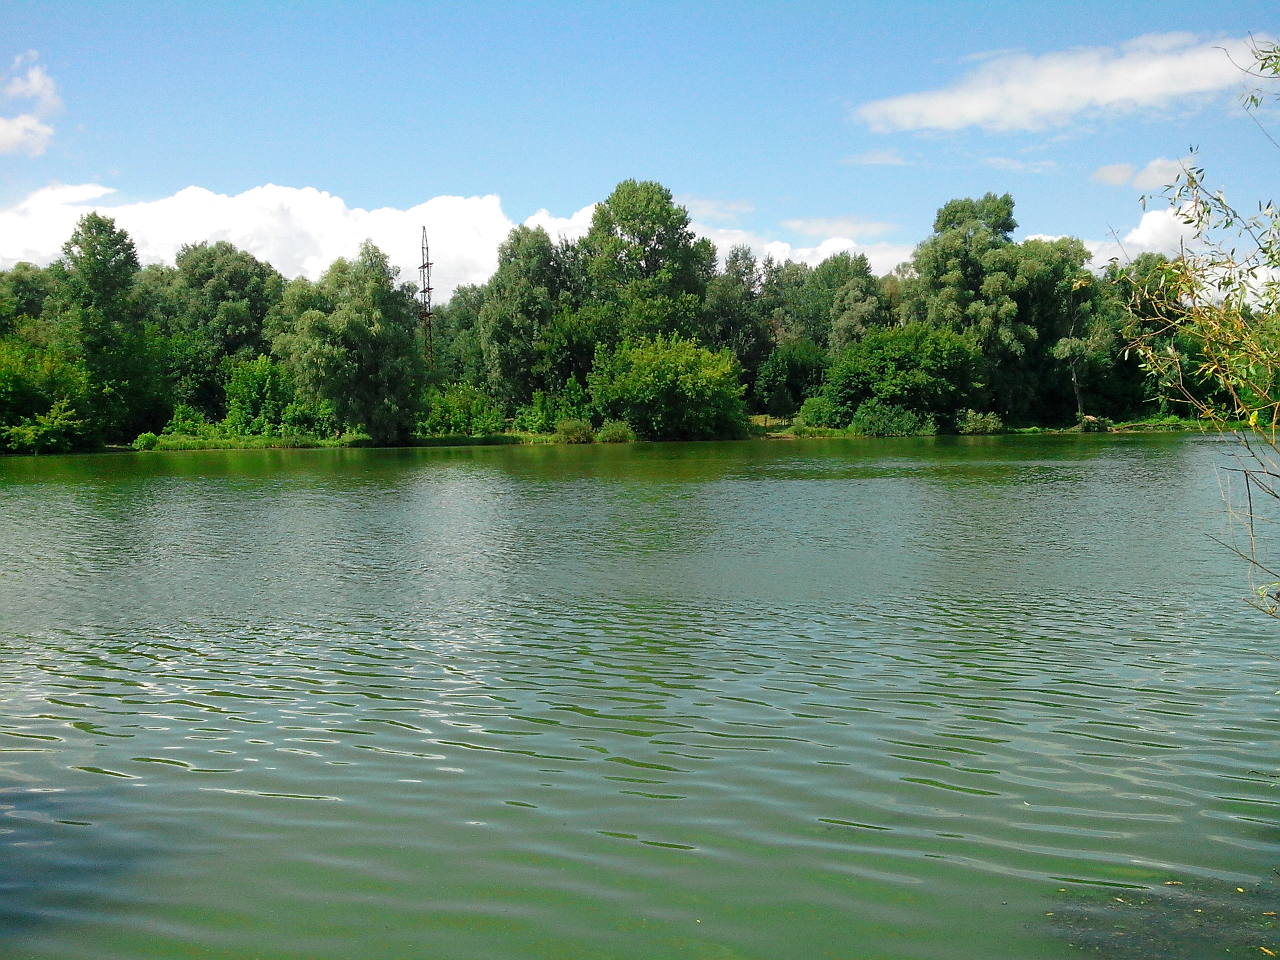
\includegraphics[width=0.93\linewidth]{chast-gorodki/darn/s_darn-IMG_20130720_144259.jpg}
\end{center}

На Березку, привлеченные клочками песчаного пляжа, ездят отдыхать из Быковни и ДВРЗ, да и со всего Киева. Обочины окрестных лесных дорог служат свалкой для разного строительного мусора. На одной из таких я нашел множество разбитых табличек с кладбища домашних животных. Озеро окружено соснами да березами. Березняк стоит на темной, торфяной почве и здорово обжит комарами, сосны же вгрузли корнями в солнечный песок. Со дна Березки тянутся водоросли, в которых запутываются купальщики. Вода часто цветет густой зеленью, будто туда вбухнули тонну акварели. Ручей, а собственно Дарница, от Плеховских болот присоединяется к озеру в восточной его части, посредством бетонного желоба.

Дарница за Ялынкой вошла в систему мелиоративных каналов в 1930-х. Уже тогда речное русло начали спрямлять, заключать в укрепленные берега, и отводить в водосборы других рек.

\newpage

Из озера Берёзки Дарница вытекает по двум совершенно разным руслам.

Примерно из северной точки (немного восточнее) Березки выходит канал, что очень скоро раздваивается. Одно русло идет прямо через лес на запад к улицам Попудренко и Мурманской. К этому руслу легко выбраться, свернув в лес напротив супермаркета «Новус» на Попудренко. Оно захламлено шинами и порой пересыхает – зависит от уровня воды в Березке.

\begin{center}
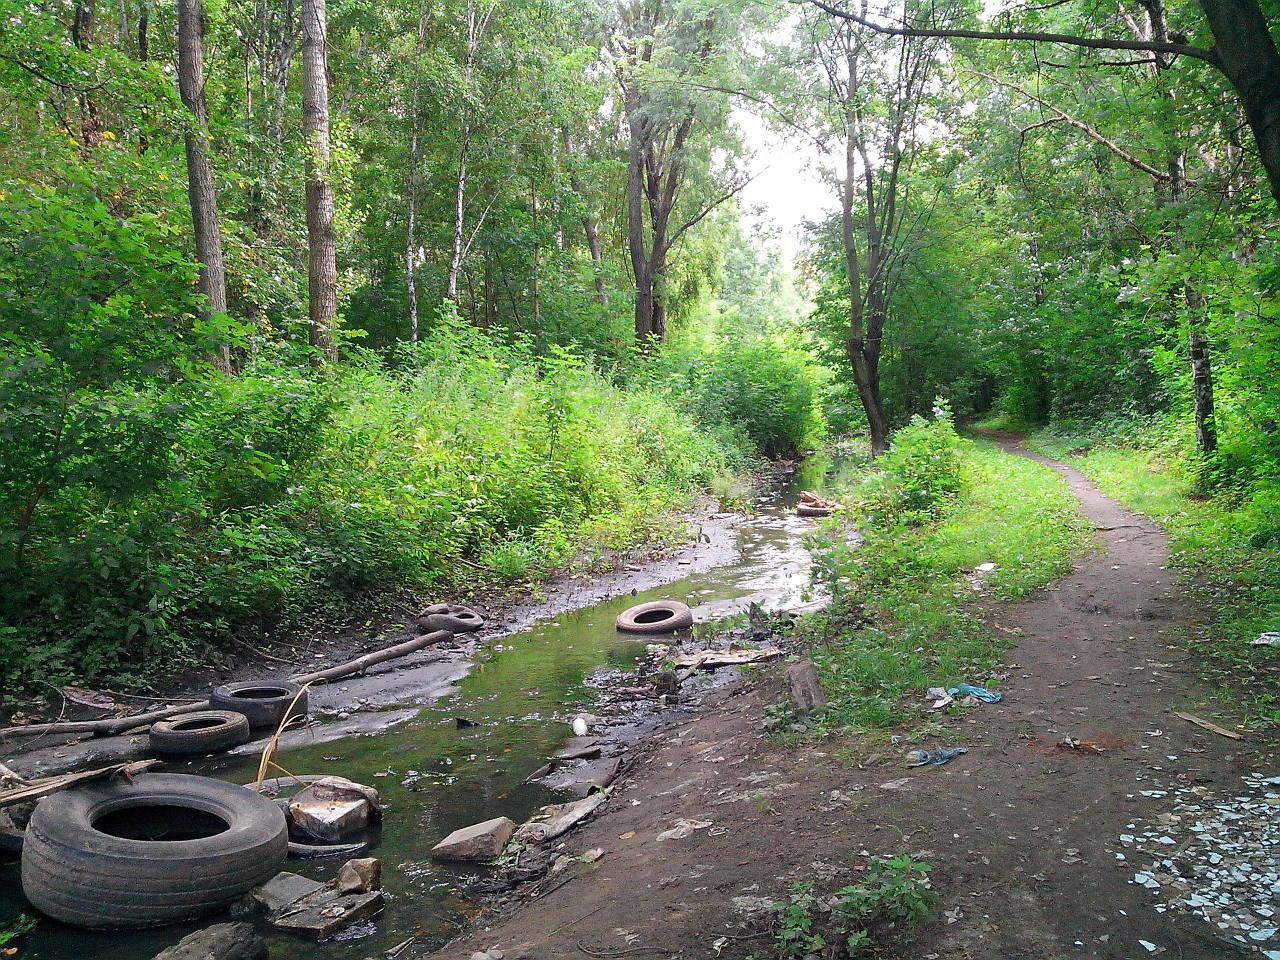
\includegraphics[width=\linewidth]{chast-gorodki/darn/s_darn-IMG_20130720_141133.jpg}

\textit{Снимок 2013 года.}
\end{center}

Сие русло тоже разветвляется. Один канал питает озеро за типографией «Блиц-принт» (что к востоку от станции метро «Лесная»), другой сворачивает резко на юг вдоль этой типографии, к заводу химикатов «Радикал», проходит между ним и лесом, и затем на юг же, мимо железнодорожной станции «Лиски»\footnote{Станцию построили для нужд Дарницкой промзоны к северу от одноименного района, возникшего на месте болота Лиски (Лески), лежавшего по историческому руслу Дарницы. Близ болота в 20 веке возник одноименный хутор. Точно на его месте теперь частный сектор между улицами Станюковича и Сновской. Местность на юго-запад оттуда, между улицами Пражской, Азербайджанской и Алма-Атинской, считалась Старой Дарницей.}, огибая ее восточную сторону. Вообще канал от Березки к «Блиц-Принту», потом через Лиски – это всё примерно по ходу старого русла Дарницы и болот вдоль него. Болота частично еще живы.

% Район же находится между станцией и Старой Дарницей, и плавно переходит в последнюю. Скажем так – Лиски это частный сектор в окрестностях улиц Калачёвской и Новаторов. Граничит с промзоной. Добраться в Лиски можно трамваем с Ленинградки на ДВРЗ. Выйти на остановке «Профсоюзная».}

На краю поселка ДВРЗ, у последних номеров улицы Олексы Довбуша, канал сворачивает на запад. Тут русло канала сохраняется неизменным с конца тридцатых годов. Оно направляется к улице академика Бутлерова, пересекает ее и заходит на территорию Дарницкой ТЭЦ. На Бутлерова Дарницу, весьма в том месте вонючую химикатами, можно пощупать около моста над нею. Русло с одной и другой стороны моста уходит под ограды. К открытой речке проще подобраться со стороны заброшенных железнодорожных путей, идущих от Киев-Лиски на север.

А следуя вдоль ТЭЦ на юго-запад, на пути к пересечению с Красногвардейской, канал прячется в коллектор\footnote{50°26'36"N 30°38'32"E}.

К юго-западу от Дарницкой ТЭЦ раньше, с 19 века и до строительства ТЭЦ в 1950-х, было большое (в 1930-х длина более 700 метров, ширина около 400) озеро Дарница, откуда река руслом (а позже новым каналом) протекала далее. Озеро, по нынешним меркам, охватывало самый северо-западный край ТЭЦ, промзону у перекрестка Павла Усенко с Красногвардейской, и до перекрестка Азербайджанской с Пражской. Вот там, за Азербайджанской номер 1, еще в 2008 году было небольшое озерцо – остаток прежнего Дарницкого! Нет уже и его. А ведь еще в начале 21 века местные жители вроде бы добились от государства решения на устройство парка вдоль русла Дарницы от Пражской и до самого Харьковского шоссе. Увы.

Вероятно, раньше Дарницкое озеро было еще больше, чем в первой половине 20 века. На карте 1799 года на нем заметны два острова. Я знаком с этой картой отрывочно и не могу соотнести размер озера с чем-либо, кроме тогдашней Кухмистерской слободы. Видимая на куске карте часть озера была эдак впятеро больше площади слободы. Тогда же, от озера речка протекала дальше на запад, примерно в сторону слободы, но забирая к югу. Вдоль западного берега озера шла дорога, по ней мост через вытекающую из озера речку, на речке – два пруда, у самого моста – «шинок Дарница», а к северу оттуда по дороге же – «трактир городской именуемый Красный».

А ныне, нырнув под Пражской, течет Дарница дальше в подземном коллекторе вдоль улицы Лохвицкой, прямо под новостройками жилищных комплексов «Родинний затишок», «Флагман», «Новая волна», «Стародарницкий». В этом месте и хотели парк вдоль речки. Подобный ход Дарницы справедлив по карте РККА 1930-х, а вот согласно Шуберту, в середине 19 века русло лежало значительно западнее. Ошибается карта Шуберта или русло переместилось?

Здесь вдоль него, на 2016 год – теснимый небоскребами и гаражными кооперативами сохраняется еще частный сектор по улицам Сосницкой, Краснокутской, Двинской и смежным с ними. Не редкость кривые заборы с калитками. Встречаются и двухэтажные многоквартирные домики.

\begin{center}
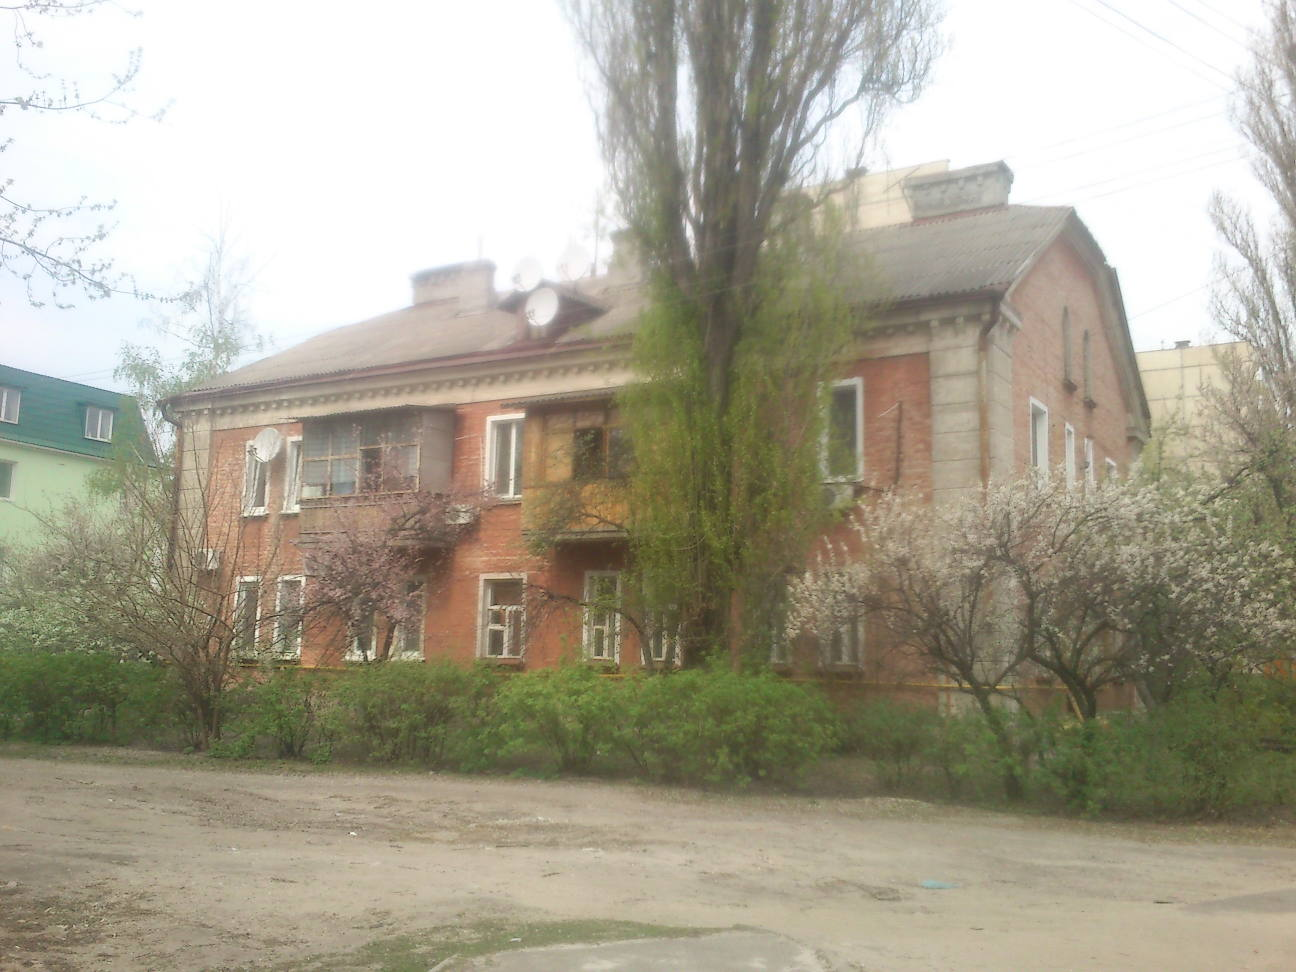
\includegraphics[width=0.85\linewidth]{chast-gorodki/darn/s_darnica-DSC_0022.JPG}

\textit{Старая Дарница 2013 год.}
\end{center}

Селиться тут стали в начале 1950-х, а до того был лес. Это место относится к Старой Дарнице. А Новая Дарница – на юг от железной дороги, станции «Дарница», где современный квартал между Харьковским шоссе, Ялтинской и Привокзальной.

\begin{center}
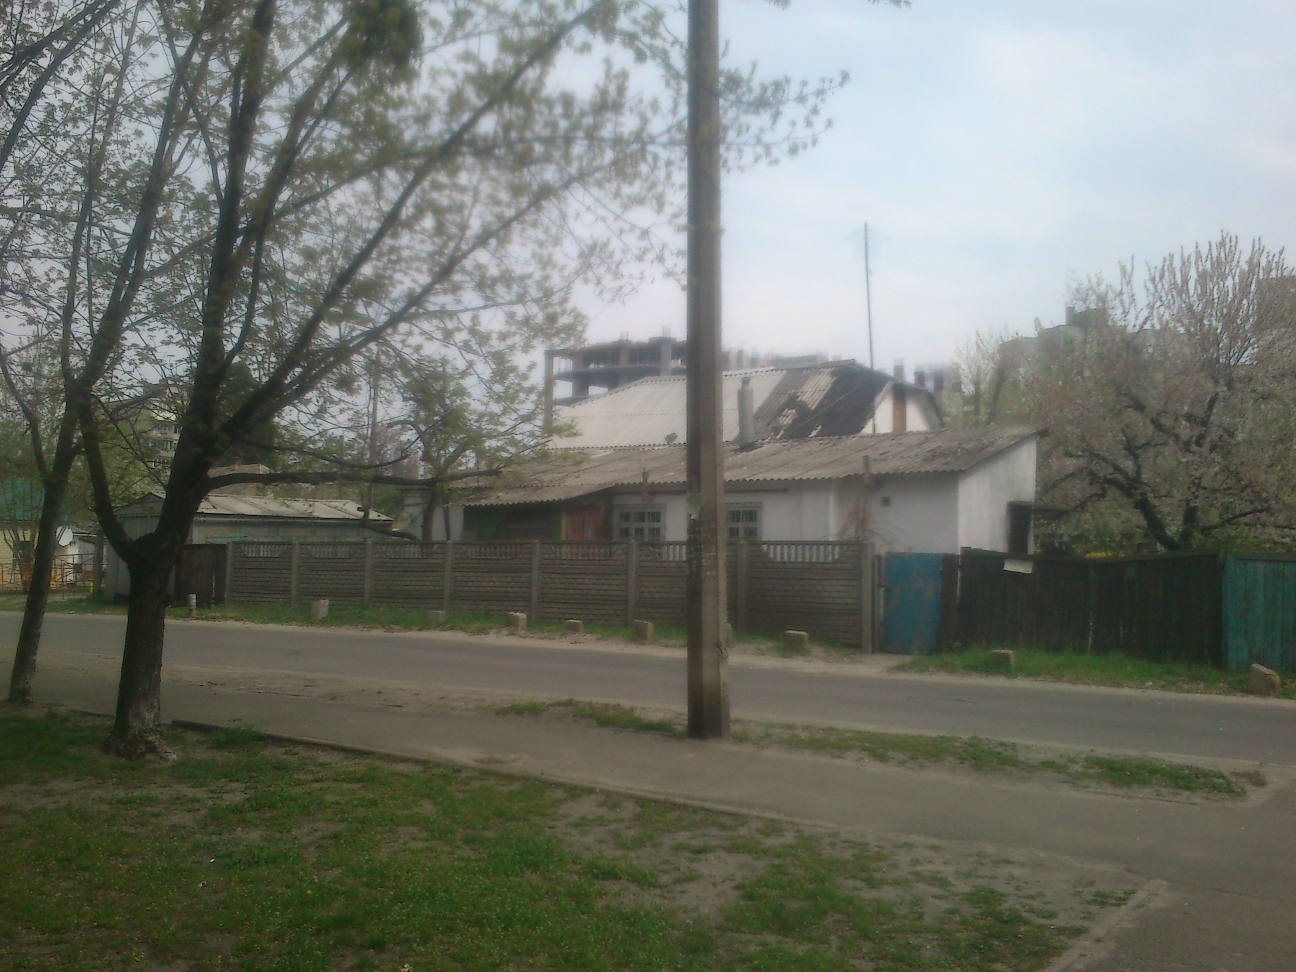
\includegraphics[width=\linewidth]{chast-gorodki/darn/s_darnica-DSC_0020.JPG}

\textit{Старая Дарница, 2013 год.}
\end{center}

Пройдя под Харьковским шоссе, речка Дарница выбирается на поверхность по улице Фанерной, за институтом химии\footnote{50°25'50.5"N 30°38'01.6"E}. К тому времени она стала полноводней. Приблизившись к железной дороге, речка снова уходит в коллектор, но какие-то соки продолжают питать перекроенную насыпями местность, образуя «болото Серой цапли» (часть прежнего русла Дарницы), и воспетый экологами «реликтовый Мокрый лес»\footnote{50°25'34.05"N 30°37'34.38"E} по другую от болота сторону насыпи. В 2013 году там остановился цыганский табор, и Мокрый лес превратился в огромный нужник и мусорную свалку.

\begin{center}
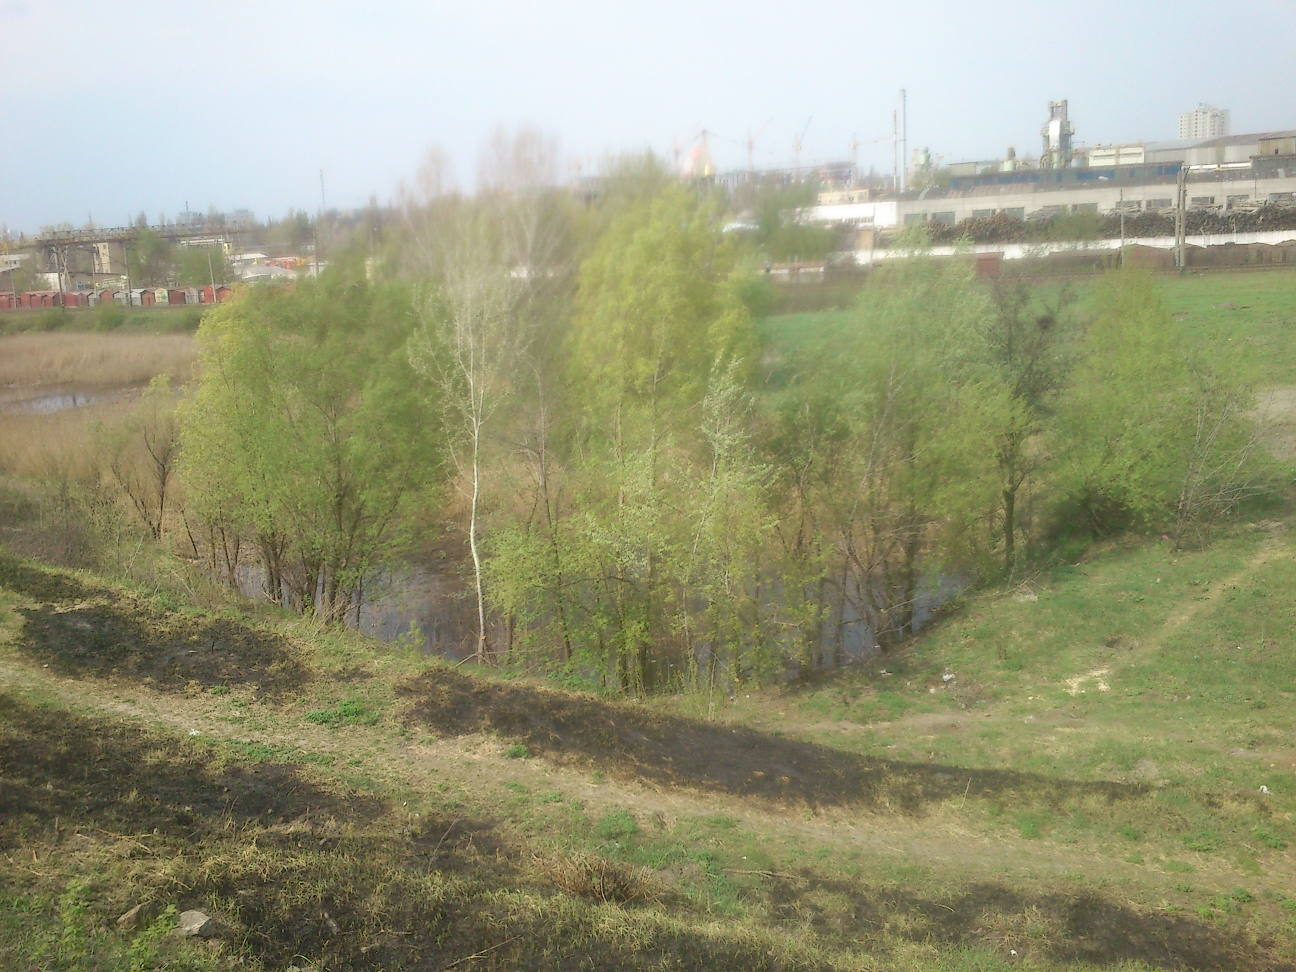
\includegraphics[width=\linewidth]{chast-gorodki/darn/s_darnica-DSC_0026.JPG}

\textit{Болото Серой цапли, 2013 год.}
\end{center}

Оба названия современны, кажется, в ходу с семидесятых годов.

Дарница на этом протяжении взята в коллектор и выходит оттуда западнее, у начала Канальной улицы и перекрестка с проспектом Григоренко. В коллекторе она смешивает воды с мутным потоком, идущим вдоль озера Прорвы по прорытому на рубеже нулевых каналу стока воды из озера Солнечного.

Близлежащее озеро Жандарка, окруженное уже не частным сектором, а высотками, за десятилетие до 2014 года полностью изменило форму и размеры в связи с перепланировкой местности. Частный сектор с улочками Тальновской, Внешней, Зоотехников, Батуринской исчез, там сейчас новостройки, из старых улиц сохранились только Днепровая и Ивана Бойко. К востоку от Бойко был и остается длинный водоем с заводями (его видно с юго-западной стороны перекрестка Здолбуновской и Григоренка), а вот на месте современного здоровенного, позеленевшего озера Жандарки еще в конце первого десятилетия 21 века протекал ручей. Отмотав время еще на 20 лет назад, к 1990-м, мы обнаружим вместо «длинного водоема» ручей с цепью прудов на нем. Как всё изменилось!

Я не зря об этом пишу. Ведь ручей был некогда продолжением нижнего течения Тельбина, продолжаясь до Осокорков, а как дальше – не ведаю.

Но вернемся к Дарнице.

Канал вдоль Канальной улицы следует на восток, мимо станции «Левый берег» и шумного шоссе. Зеленые бурьяны, закрывшие собой берега, скрыли горы свезенного сюда строительного мусора, где попадались старинные кирпичи. По другую сторону от шоссе, через реку, за старыми деревьями приумножаются гаражи и промзона.

Я помню это место в восьмидесятых. Лето, синее высокое небо, полустанок, а под насыпью, на пустыре – площадка для дрессировки собак, и обросшее камышом озеро Нижний Тельбин.

А в 2013 году, по левому берегу Нижнего Тельбина –  той части канала, что прокопана ближе к Днепру – тянется, между водой и улицей Канальной, пустырь, успевший у берега порасти деревьями. Чахлая трава щедро усеяна хламом. К озеру со всех сторон подбирается стройка. Строители ловят рыбу, еще какой-то мужичок ловит рыбу, неведомо кто жжет костер из резины. 

Мы заканчиваем снимать очередную ходку «Киевской Амплитуды», полчаса назад попали в бешеную пылевую бурю, когда даже деревья размахивали ветками, чтобы отогнать ветер. До транспорта идти еще порядочно, к набережной Днепра и Русановке. Я растер себе ноги берцами\footnote{Которые убились только осенью 2016 года при исследовании с Колей Арестовым склонов ботсада на Зверинце.}, зато в них удобно было шагать по камням около рельсов, где я подобрал несколько кусков кремния, заподозрив в них первобытные орудия. Тучи исчезли, засветило солнце.

От Набережной мы перешли на другую сторону улицы, и я пошел к маршрутке, а в камере осталось снятое за день видео, да в мобилке – несколько расплывчатых снимков, потому что там накрылась матрица, и фотографии получались с налетом нежной грусти.

\begin{center}
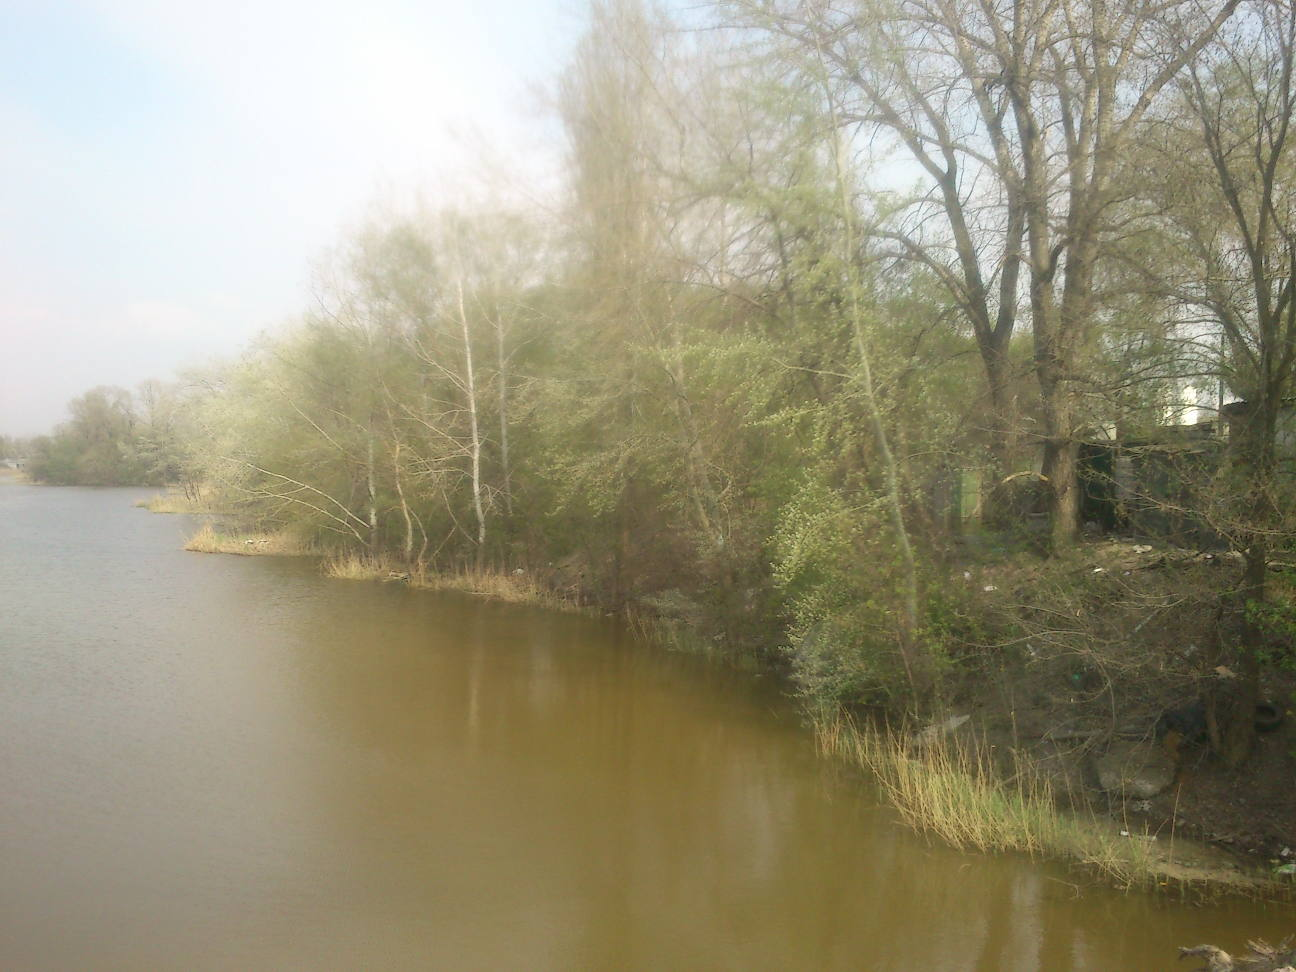
\includegraphics[width=\linewidth]{chast-gorodki/darn/s_darnica-DSC_0028.JPG}

\textit{2013. Нижний Тельбин.}
\end{center}

Вода из Нижнего Тельбина уходит в Днепр, но это не конец Дарницы, а лишь одно из устий. Ведь существует вторая ветвь канала от озера Берёзки!

Два съемочных дня ушли на его исследование, хотя в разное время я был на его отрезках и раньше, а порой бывал и позже.

Второй канал идет от Березки на северо-запад, к западной границе посёлка Быковни, где еще в середине прошлого века по обе стороны шоссе было два озера.

Канал ныряет под Броварское шоссе и обретается на коротком отрезке по улице Кузбасской, после чего в коллекторе следует на северо-запад, пересекает улицу Киото и выходит рвом в Быковнянском лесу. Там речка Дарница с переменным успехом течет в направлении Лесного массива. Вода в канале зеленая, иногда невозможно понять, стоит она или движется. В 2013 году с севера канал получал приток – ручей с примесью железистых частиц. К 2016 году этот ручей высох.

В окрестностях станции метро Лесная, в лесу, канал поворачивает вдоль улицы маршала Жукова и прячется там в коллектор, чтобы выйти наружу в противоположной части Лесного массива, за автоматической телефонной станцией на Милютенко, 29.

Это положение дел на 2016 год. В лесу поныне остались пересохшие мелиоративные каналы, наибольший из которых заканчивается у южного конца Лесного кладбища. Мы сейчас подобрались к теме, которую я широко буду развивать в главе о Радунке – про водную систему на Троещине, Воскресенке, Радужном. Так получилось, что воды Дарницы и мелиоративные каналы искусственно вмешались в жизнь этой местности, и моя задача – попытаться размежевать исконные речки и канал Дарницы.

От Милютенко канал шпарит на северо-запад по местности болота Казенного, к 21 веку весьма пересохшего, но кое-где сохранившегося. В середине 20 века тут было большое озеро, окруженное болотом. Оно питалось от ручья, что начинался чуть северо-западнее перекрестка улицы Жукова и Лесного проспекта. Ручей ныне смешивается с речкой Дарницей и составляет б\'ольшую часть объема воды в канале, если не всю, ведь в последние годы уже на приближении к Лесному, мелиоканал от речки Дарницы почти высох. Поэтому именование канала Дарницей дальше, за Лесным, весьма условно.

На участке леса между улицами космонавта Волкова, Братиславской и Крайней, среди березняка – водянистые, буйно заросшие торфы с кочками да ручейки. По этому-то Казенному и течет в канале вода.

Сначала, по выходу из коллектора у телефонной станции, она страшная – черная. Набросано много автомобильных шин и прочего хлама. Стоит гнилая вонь. Надо думать, черный цвет – это размытый болотный торф. Поперек леса, с востока на запад до Куликово – старая грунтовка с деревянными столбами\footnote{От 50°29'1.17"N 30°37'25.18"E до 50°28'47.33"N 30°36'36.54"E, и далее на север. У канала и под Братиславской дорога прерывается.}. 

Еще более старая дорога, кажется многовековая, находится в лесу между улицей космонавта Волкова и Лесным кладбищем, прерванная ныне последним, и сворачивает потом на восток по высокому берегу Алмазного озера, бывшего болота, и дальше в направлении Броваров. Шлях этот виден даже на плане Шуберта, однако уцелел по наше время не полностью.

Но вернемся к каналу. Ближе к улице Крайней слышны голоса людей, люди там заняли участок леса и всячески назойливо отдыхают. За полторы сотни метров от перекрестка Братиславской с Крайней, Дарница уходит в коллектор под Воскресенкой. Диггеры плавали по нему в надувной лодке.

Местность вдоль южной части Крайней и оттуда к Петра Запорожца и Курнатовского была прежде занята болотом Куликово. Лес на восток от Братиславской и сейчас, посуху, перекроен каналами да гатями. А Куликовым теперь называется район в треугольнике Братиславской – Курнатовского – Стальского, застроенный в 1980-1982 годах девятиэтажками. Во второй половине прошлого века Куликовым считалось еще и место, где нынче Троещинский вещевой рынок. Прежде болото северной развилкой достигало его южной и восточной границ.

В первой половине 20 века болото Куликово составлялось из двух рукавов. Один, частично сохранившийся, лежит вдоль улицы Крайней. Другой начинался у теперешнего дома по адресу Братиславская, 18Б и шел между шоссейной часть улицы и домами, где сейчас полоса поросшего деревьями и травой пустыря. 

На юго-запад от перекрестка Крайней и Братиславской (где оба русла смыкались), примыкая к району Куликово, есть метров двух глубиной ложбина вдоль леса, оставшаяся от общего болотного русла. В ней, ее приближенной к перекрестку части, изредка появляется вода и имеет течение на юг. Всё носит следы облагораживания – кажется, в советские времена тут был оборудован даже пляжик (остались бетонные ступени). Сохранились остатки неких хозяйственных сооружений – перегородки с дверцами.

В конце тридцатых или самом начале сороковых годах двадцатого века там проходил мелиоративный канал, до места, где сейчас роддом около перекрестка Курнатовского и Петра Запорожца. Туда же в конце тридцатых проложил новый (взамен прежнего) канал от проточного озера на юге отсюда.

Это возле станции метро «Дарница» есть парк Победы\footnote{В середине 1980-х мы пару раз ездили в гости к знакомым, что жили в огромном полукруглом доме около этого парка, через улицу. Выбрались погулять и в парк, где стоит семиметровый курган Бессмертия (первое и полное название «Курган Бессмертия в память о тех, кто отдал свою жизнь за власть Советов»), торжественно открытый, как и парк, в 1967-м. Он насыпан из земли с солдатских и партизанских могил. Основание кургана – в виде пятиконечной звезды, хотя сам выглядит пирамидой. Так вот, знакомые рассказали, что по ночам над курганом наблюдают странное свечение.}. До парка, здесь загнивал заболоченный ручей с несколькими озерцами по нему, хотя еще в 1930-х там было большое заболоченное озеро\footnote{На карте РККА 1930-х на западном берегу обозначен некий «Питомник».}, занимавшее пространство от современной улицы генерала Жмаченко до жилого комплекса «Парковые озера». Русло этого озера, как хорошо прослеживается на старых картах, да и на местности – продолжение того же древнего водоема, часть которого заняло болото Куликово.

В 2004 году ручей превратили, в пределах парка в – ну как сказать – полевую реку длиной один километр. Небольшое течение, вода понемногу выходит через трубу из северной части водоема, движется под проспектом Алишера Навои и ровным наземным каналом дальше на север, через лес, вдоль Курнатовского, к больнице и роддому. Не доходя до него, уходит в коллектор. И в нем уж соединяется с водами Дарницы.

Вторгнувшись по Воскресенскому коллектору в чужой водосбор, водосбор Радунки, Дарница под землей идет севернее Радужного озера, на запад, минует очистные сооружения на улице Петра Вершигоры, проходит под противопаводковой дамбой и вскоре, за озерцом у пустыря, впадает в залив Десёнку.

%Вот я и закончил рассказ о Черторые, Тельбине и Дарнице. О последней просто к слову получилось, да и всё равно пришлось бы потом объяснять, откуда взялась дополнительная вода там, где ее раньше не было. Мог и короче, без слободок, да про них знают мало, как не поведать? Хорошо хоть о мото-трамвае развить мне помешали иллюстрации, а то бы еще добавил, что линию его в конце двадцатых таки электрифицировали, и по мосту Бош перед войной ходил уже лектрический трамвай, а не переделанные на рельсовый ход грузовики.

%Набравшись сил, продолжу свою повесть о левобережных реках, подбираясь к Городку, хотя не он здесь самое любопытное.
